\chapter{Cache-oblivious B-trees}
\label{chapter:cob}
The \emph{cache-oblivious B-tree} introduced by \cite{cobt}
is a~data structure which replicates the asymptotic performance of B-trees
in a~cache-oblivious setting.
\textsc{Find}s and updates on cache-oblivious B-trees require $\Theta(\log_B N)$
\footnote{Strictly speaking, the bound is $\Theta(1+\log_B N)$
	because we perform $\O(1)$ block transfers even when $B\in\omega(N)$.
	We decide to use the reasonable assumption that
	$B<N$ to simplify some bounds in this section.}
amortized block transfers, which is similar to cache-aware B-trees.
Scanning a~range of $t$ keys also takes $\Theta(\log_B N+t/B)$ time.

The original cache-oblivious B-tree as described in \cite{cobt} used
weight-balanced B-trees. We implement a~simplified version of the structure
from \cite{brodal01}, which is composed of three components.
The \emph{van~Emde Boas layout} of binary trees is a~way of cache-obliviously
maintaining full binary trees in memory such that reading or updating any
root-to-leaf path in root-to-leaf or leaf-to-root order takes $\Theta(\log_B N)$
block transfers.
Then, the \emph{packed memory array} lets us store a~``cache-oblivious linked
list''. The items of this ``linked list'' will represent key-value pairs,
and later groups of key-value pairs.
The packed memory array has fast updates in the amortized sense. Inserting
and deleting items overwrites $\Theta(\frac{\log^2 N}{B})$ amortized memory
blocks.
Finally, we combine the two previous parts with \emph{indirection} to obtain
the desired $\Theta(\log_B N)$ time for \textsc{Find}, \textsc{Insert} and
\textsc{Delete}.

\section{The van~Emde Boas layout}
The van~Emde Boas layout is a~way of mapping the nodes of a~full binary
tree of height $h$ to indices $0\ldots 2^h-2$. There are $N=2^h-1$ nodes.
Other layouts of full binary trees include the BFS or DFS order.

Surprisingly, the van~Emde Boas layout was not invented by van~Emde Boas.
The name comes from the earlier \emph{van~Emde Boas priority queue},
which was invented by a~team led by Peter van Emde Boas \cite{van-emde-boas}.
The van Emde Boas priority queue uses a~height splitting scheme similar
to the van Emde Boas layout. The cache-oblivious application of this idea
was devised in \cite{veb-layout}.

The advantage of storing a~full binary tree in the van Emde Boas layout
is that is lets us read the sequence of keys from the root to any leaf
using $\Theta(\log_B N)$ block transfers, which matches the \textsc{Find}
cost of \mbox{B-trees} without the need to know~$B$ beforehand.
In contrast, the same operation would cost $\Theta(\log N-\log B)$ block
transfers in the BFS or DFS order.

The van Emde Boas layout is defined recursively. To find the van Emde Boas layout
of a~full binary tree of height $h$, we split the tree to bottom subtrees
of height $\lhfloor h-1 \rhfloor$ and one top subtree of height $h - \lhfloor
h-1 \rhfloor$.
The subtrees are recursively aligned in the van Emde Boas layout and then laid
out: the top tree first, followed by the bottom trees in left-to-right order.
The van Emde Boas layout of a~one-node tree is trivial.

\begin{figure}
\centering
\begin{tikzpicture}[
	every node/.style={inner sep=0, outer sep=0},
	level 1/.style = {sibling distance=7.1cm},
	level 2/.style = {sibling distance=3.5cm},
	level 3/.style = {sibling distance=1.7cm},
	level 4/.style = {sibling distance=0.8cm},
	veb_node/.style = {align=center, inner sep=0pt, text centered, circle,
		font=\sffamily, draw=black, text width=1.2em, outer sep=0pt},
	block_l0/.style = {rectangle, draw=black, dashed, inner sep=0.2cm,
		draw=gray},
	block_l1/.style = {rectangle, draw=black, densely dotted, thin, inner
		sep=0.1cm, draw=gray},
	level/.style={level distance=1.2cm}
]
	\node [veb_node] (Node0) {0}
	child{ node [veb_node] (Node1) {1}
		child { node [veb_node] (Node2) {2}
			child { node [veb_node] (Node4) {4}
				child { node [veb_node] (Node5) {5} }
				child { node [veb_node] (Node6) {6} }
			}
			child { node [veb_node] (Node7) {7}
				child { node [veb_node] (Node8) {8} }
				child { node [veb_node] (Node9) {9} }
			}
		}
		child { node [veb_node] (Node3) {3}
			child { node [veb_node] (Node10) {10}
				child { node [veb_node] (Node11) {11} }
				child { node [veb_node] (Node12) {12} }
			}
			child { node [veb_node] (Node13) {13}
				child { node [veb_node] (Node14) {14} }
				child { node [veb_node] (Node15) {15} }
			}
		}
	}
	child{ node [veb_node] (Node16) {16}
		child { node [veb_node] (Node17) {17}
			child { node [veb_node] (Node19) {19}
				child { node [veb_node] (Node20) {20} }
				child { node [veb_node] (Node21) {21} }
			}
			child { node [veb_node] (Node22) {22}
				child { node [veb_node] (Node23) {23} }
				child { node [veb_node] (Node24) {24} }
			}
		}
		child { node [veb_node] (Node18) {18}
			child { node [veb_node] (Node25) {25}
				child { node [veb_node] (Node26) {26} }
				child { node [veb_node] (Node27) {27} }
			}
			child { node [veb_node] (Node28) {28}
				child { node [veb_node] (Node29) {29} }
				child { node [veb_node] (Node30) {30} }
			}
		}
	};

	\node [block_l0,fit=(Node0)] (BlockT) {};
	\node [block_l0,fit=(Node1) (Node5) (Node15)] (BlockB0) {};
	\node [block_l0,fit=(Node16) (Node20) (Node30)] (BlockB1) {};

	\node [block_l1,fit=(Node1) (Node2) (Node3)] (BlockB0T) {};
	\node [block_l1,fit=(Node4) (Node5) (Node6)] (BlockB0B0) {};
	\node [block_l1,fit=(Node7) (Node8) (Node9)] (BlockB0B1) {};
	\node [block_l1,fit=(Node10) (Node11) (Node12)] (BlockB0B2) {};
	\node [block_l1,fit=(Node13) (Node14) (Node15)] (BlockB0B3) {};

	\node [block_l1,fit=(Node16) (Node17) (Node18)] (BlockB1T) {};
	\node [block_l1,fit=(Node19) (Node20) (Node21)] (BlockB1B0) {};
	\node [block_l1,fit=(Node22) (Node23) (Node24)] (BlockB1B1) {};
	\node [block_l1,fit=(Node25) (Node26) (Node27)] (BlockB1B2) {};
	\node [block_l1,fit=(Node28) (Node29) (Node30)] (BlockB1B3) {};
\end{tikzpicture}
% TODO: linearized figure, general figure

\caption{The van Emde Boas layout of a~full binary tree of height 5.
Boxes mark recursive applications of the construction. Note that the indices
within every box are contiguous, so at some level of detail, reading
a box will take $\O(1)$ block transfers.}
\label{fig:veb_layout_5}
\end{figure}

\begin{theorem}
In a~tree stored in the van Emde Boas layout, reading the sequence of nodes
on any root-leaf path costs $\Theta(\log_B N)$ block transfers.
\end{theorem}

\begin{proof}
First, consider only van Emde Boas layouts with $h$ a~power of two.
Examine recursive applications of the van Emde Boas construction.
The first recursion splits the tree of height $h$ into a~top tree of height
$h-\lhfloor h-1\rhfloor=h/2$ and a~bottom tree of height $\lhfloor
h-1\rhfloor=h/2$. The second recursion splits all trees of height $h/2$
into trees of height $h/4$, and so on. Denote the heights of constructed bottom
trees at recursion level $i$ as $h_i=h/2^i$.

Note that at every level of recursion, every tree is stored in contiguous
memory. Assume that any node can be stored in one machine word. A~cache block
of $B$~words accomodates $B$~nodes, so there is some level of recursion $i$
for which trees of height $h_i$ fit into a~cache block, but trees of the next
larger height $h_{i-1}$ do not. In other words, $2^{h_i}-1 < B$ and
$2^{h_i-1}-1\geq B$, from which $h_i=\Theta(\log B)$ follows.

Root-to-leaf paths contain $\Theta(\log N)$ nodes, and these nodes span
$\Theta(\frac{\log N}{h_i})$ trees of height $h_i$. Since each such tree can be
read using one block transfer, we need $\Theta(\frac{\log N}{h_i})=\Theta(\log_B
N)$ block transfers to traverse any root-to-leaf path.

If $h$ is not a~power of two, recursively generated top and bottom trees may no
longer have heights that are powers of two. However, note that if we again
divide the tree into subtrees until atomic subtrees of height $h_i$ fit into
cache blocks, almost all trees encountered on any root-to-leaf path will still
have height~$h_i$. The only exception will be the tree that contains the root,
which may have height less than $h_i$. The original argument still works:
we need $\Theta(\log_B N)$ block transfers for traversing a~root-to-leaf path,
including an $\O(1)$ added for reading the tree containing the root.
\end{proof}

The van Emde Boas layout thus makes a~fine data structure for querying static
data, but it does not allow inserting or deleting nodes. We will need
to combine it with another data structure to allow updates.

\subsection{Efficient implementation of implicit pointers}
A useful property of the van Emde Boas layout is that it is fully specified
by the height $h$ of the tree, so there is no need to keep pointers to child
nodes. The positions of left and right children of a~node can be calculated
from $h$ when they are needed.
This is particularly useful when $B$ is small and when the size of pointers
is similar to the size of keys, because not storing pointers lets us
effectively use a~higher branching factor than B-trees with explicit
pointers could.
For example, if we store 8-byte keys in a B-tree and if we align nodes to
a 64-byte cache line, each node can only store up to 3 keys. In contrast,
64 bytes of a~van~Emde Boas layout store 8 keys.
% We refer to this property of the layout as allowing
% \emph{implicit pointers}.

We will only use the van~Emde Boas order to walk in the direction from
the root node to a leaf or in reverse.
Given the \emph{van~Emde Boas ID} of a node (denoted as numbers
inside the nodes in Figure \ref{fig:veb_layout_5}),
we can easily calculate the van~Emde Boas IDs of its children by
a recursive procedure. This procedure either returns \emph{internal} node
pointers, referencing actual nodes of the tree, or it returns \emph{external}
indexes, which represent virtual nodes below the leaves, counted from left
to right.

\begin{algorithmic}
\Function {GetChildren} {$n$: node van Emde Boas ID, $h$: tree height}
	\If {$h = 1$ and $n = 0$} \Return{external (0,1)} \EndIf

	\State {$h_\downarrow \gets \lhfloor h-1 \rhfloor$} \Comment{Calculate
top and bottom heights}
	\State {$h_\uparrow \gets h-h_\downarrow$}
	\State {$N_\uparrow, N_\downarrow \gets 2^{h_\uparrow}-1,
	2^{h_\downarrow}-1$} \Comment{Calculate top and bottom tree sizes}

	\If {$n <  N_\uparrow$}
		\State $\ell, r \gets$ \Call{GetChildren}{$n$,$h_\uparrow$}
		\If {$\ell$ and $r$ are internal}
			\State \Return{internal ($\ell$,$r$)}
		\Else\Comment{$\ell$ and $r$ point to bottom tree roots}
			\State \Return{internal
				($N_\uparrow+\ell\cdot N_\downarrow$,
				$N_\uparrow+r\cdot N_\downarrow$)
			}
		\EndIf
	\Else
		\State {$i \gets (n-N_\uparrow) / N_\downarrow$}
			\Comment{The node $n$ lies within the $i$-th bottom tree.}
		\State {$b \gets N_\uparrow + i\cdot N_\downarrow$}
			\Comment{$b$ is the root of the $i$-th bottom tree.}
		\State $\ell,r\gets$ \Call{GetChildren}{$n-b$, $h_\downarrow$}
		\If {$\ell$ and $r$ are internal}
			\State \Return{internal ($\ell+b$, $r+b$)}
		\Else
			\State {$e \gets 2^{h_\downarrow}$} \Comment{Adjust
				indices by $e$ external nodes per bottom
				tree.}
			\State \Return{external ($\ell+i\cdot e$, $r+i\cdot e$)}
		\EndIf
	\EndIf
\EndFunction
\end{algorithmic}

The cost of this procedure in the cache-oblivious model is $\O(1)$, because
it can be implemented using constant memory by modifying the tail recursion into
a loop. Unfortunately, on a real computer, this is not quite the case --
every call of this procedure performs $\Theta(\log\log N)$ instructions and
the cost of calling this procedure $\Theta(\log N)$ times between the root
and a leaf is not negligible compared to the cost of memory transfers.
Indeed, this calculation of implicit pointers can become the performance
bottleneck of the cache-oblivious B-tree.
This can be slightly alleviated by caching the results for trees of small
height, which allows us to stop the recursion early.

As described in \cite{brodal01}, at the low cost of precomputing $\O(h)$
items for every height $h$ of the binary tree, we can perform root-leaf
traversals in constant time per traversed level.

The main observation is that for any node in a fixed depth $d$,
performing the recursive construction until the selected node is the root
of a bottom tree will progress through the same sizes of top and bottom trees.

For every depth $d\in[2;h]$, let us precompute the size $B[d]$ of
bottom trees rooted in depth $d$, the size $T[d]$ of the corresponding
top tree and the depth $D[d]$ of the top tree's root. The data takes $\O(\log
N)$ memory and it can be computed in $\O(\log N)$ time by an iterative procedure.
Table \ref{tab:depth_data_example} shows the values of these arrays
for the 5-level van Emde Boas layout shown from Figure \ref{fig:veb_layout_5}.

\begin{table}[h]
	\centering
	\begin{tabular}{r|r|r|r}
		$d$ & $B[d]$ & $T[d]$ & $D[d]$ \\
		\hline
		0   & --     & --     & --     \\
		1   & 15     & 1      & 0      \\
		2   & 1      & 1      & 1      \\
		3   & 3      & 3      & 1      \\
		4   & 1      & 1      & 3
	\end{tabular}
	\caption{$B[d]$, $T[d]$ and $D[d]$ for the 5-level van Emde
	Boas layout.}
	\label{tab:depth_data_example}
\end{table}

While traversing a root-to-leaf path, we shall maintain the depth
$d$ of the current node $X$, the index $i$ of the current node in BFS order
and an array $Pos[j]$ of van Emde Boas order indices of nodes passed in every
depth $j<d$ during this traversal.

As the bits of the BFS index $i$ correspond to left and right turns made during
the traversal, the $\log(T[d]+1)$ least significant bits of $i$ are the
index of the unique bottom tree rooted by the node $X$. Because $T[d]$ is
always in the form $2^k-1$, we can find those bits quickly by calculating
$i \And T[d]$.

Because the current node $X$ is the root of the $(i \And T[d])$-th
bottom tree of size $B[d]$ after a top tree of size $T[d]$ rooted in
$Pos[D[d]]$, it follows that the van Emde Boas index of the current node can be
calculated in $\O(1)$ time as:
$$Pos[d]=Pos[D[d]] + T[d] + (i \And T[d]) \cdot B[d]$$

Our root-to-leaf traversal starts by setting $i\gets 0, d\gets 0, Pos[0]=0$.
Navigation to the left or right child of the current node is performed
by updating the BFS index $i$ (setting it to $2i+1$ or $2i+2$ respectively),
incrementing the depth $d$ and calculating the new $Pos[d]$.
We can also return one level higher by reversing the update of $i$ and
decrementing $d$.

In our root-to-leaf traversals, reading the value of a non-leaf node $N$ will be
followed by reading the value of its right child $R$. Based on the value in
$R$, we will then either descend further below $R$, or we will descent into
the subtree below $N$'s left child $L$.
We can slightly optimize this access pattern by calculating $Pos[d]$ for $L$
from $Pos[d]$ for $R$ by simply subtracting $T[d]$, because $B[d]$ will
decrease by 1. This saves us one relatively expensive multiplication
instruction whenever moving to the left sibling.

\begin{figure}
\centering
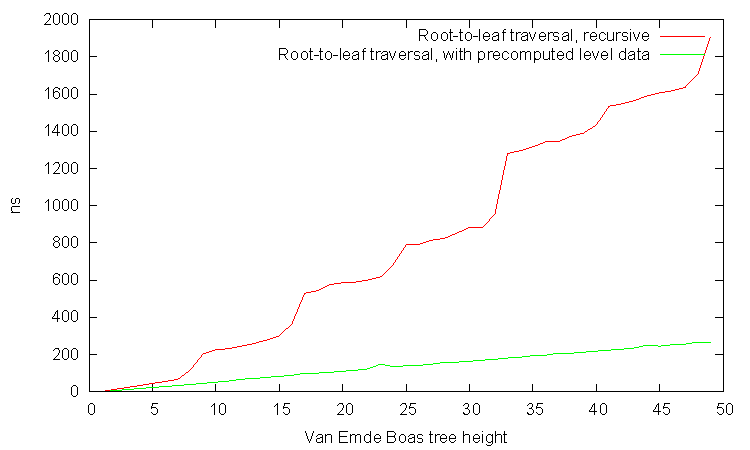
\includegraphics{img/veb-drilldown-speed}
\caption{Average time for computing node pointers in root-to-leaf traversals
	of van Emde Boas layouts, implemented trivially and with precomputed
	level data.}
\label{fig:veb_drilldown_speed}
\end{figure}
As evident from Figure \ref{fig:veb_drilldown_speed}, using precomputed level
data saves a considerable amount of computation, especially with deeper
van~Emde Boas layouts.

\section{Ordered file maintenance}
Ordered file maintenance algorithms maintain $N$ items stored in a physical
array of size $\O(N)$. Aside from reading from any slot in the array,
we can ask the algorithm to \textsc{Insert} a new item before or after
a given index in the array, and \textsc{Delete}(\emph{index}), which deletes
the item at a given index. Updates are allowed to move elements of the array,
but the relative order of all stored items must remain the same.

While the interface is similar to a simple linked list, storing the items
in a~contiguous array of size $\O(N)$ lets us scan a range of size $k$ using
only the optimal $\Theta(k/B)$ block reads, which improves upon linked lists
by a~factor of $B$.

To give the maintenance algorithm some freedom, empty gaps of up to a~constant
maximum size may be present between two adjacent items in the array. Without
gaps, \textsc{Insert} and \textsc{Delete} would have to be implemented
by shifting elements to the right or left in $\Theta(N/B)$ block transfers.

The \emph{packed memory array} is a~data structure that maintains an ordered
file. Updates (\textsc{Insert}s and \textsc{Delete}s) of a~packed memory array
rewrite a~contiguous range of amortized size $\Theta(\log^2 N)$.
Thanks to the range being contiguous, updates will incur
$\Theta(\frac{\log^2 N}{B})$ amortized block transfers.

The array is divided into logical \emph{leaf blocks} of constant size
$\O(\log N)$. A~\emph{virtual full binary tree} is built above those leaf
blocks. Every node of this binary tree represents the range covering all
the leaf blocks below. This tree is only conceptual -- it is never stored
in memory. The root of the virtual tree is the range covering the entire
ordered file, and the children of any range are its left and right halves.
For simplicity, the virtual tree assumes that the number of leaf blocks
is $2^x$. Any ranges that do not fall within the actual backing array
are ignored.

To properly describe the structure, we need to define some terms. The
\emph{capacity} of a~certain range of the array is its size and the
\emph{density} of a~range is the number of items present in the range divided
by its capacity.
The packed memory array maintains certain bounds on the densities of subranges
of the array.

The densities in the leaf blocks are kept between $1/4$ and 1.
If an update keeps the density of the leaf block within thresholds, we perform
the update by rewriting all $\Theta(\log N)$ items of the leaf block.
When the range covering the leaf block becomes too sparse or too dense, we
walk up the virtual tree of ranges until we find a node that fits our density
requirements. The parent range is obtained by doubling the size of the child
range, extending the child on the left or on the right (depending on
whether the child range was a right or left child of its parent range).

The density requirements become stricter on larger ranges.
In particular, the density of a node of depth $d$ within a tree of height $h$
is kept between $\frac{1}{2}-\frac{1}{4}\frac{d}{h}$ and
$\frac{3}{4}+\frac{1}{4}\frac{d}{h}$.
\footnote{The constants are arbitrary and control the tradeoff
between memory consumption and time complexity of rebuilding.}
When we find a node that is \emph{within threshold}, we uniformly redistribute
the items in its range. If no such node exists, we resize the entire structure
by a~constant factor, which lets us amortize the costs of this resizing to
a multiplicative constant.

We claim that while this redistribution may reorganize a range of size up
to $\O(N)$, the redistribution of a node puts all nodes below it well within
their thresholds, so the next reorganization will be needed only after many more
updates.

The search for a node to redistribute is implemented as two interspersed scans,
one extending the scanned range to the left, one to the right. The
redistribution can be done by collecting all items in the array on the left side
of the array using a left-to-right scan, followed by a right-to-left scan
putting items into their final destinations. Thus,
redistributing a range of $K$ items takes $\Theta(K/B)$ block transfers.

% TODO: figure of redistribution

\begin{theorem}
The block-transfer cost of an update of the packed-memory array
is $\Theta(\frac{\log^2 N}{B})$ amortized.
\end{theorem}

\begin{proof}
Suppose we need to redistribute some node $X$ of depth $d$ after performing
an insertion. Since we are redistributing this node, it is within threshold,
but one of its children, say $Y$, is not.
Therefore the density of $X$ is at most
$\frac{3}{4}+\frac{1}{4}\frac{d}{h}$, while the density of $Y$ is more than
$\frac{3}{4}+\frac{1}{4}\frac{d+1}{h}$. After we redistribute the items
within~$X$, the density of $Y$ will drop by $1/h$. Thus, if we denote
the capacity of $Y$ as $|Y|$, we will need to insert at least $|Y|/h$ items
under any child of $X$ before we need to rebalance $X$ again.
Thus, we can charge the $\O(|X|)$ cost of redistributing $X$ to the
insertions into $Y$, which gives us amortized $\O(\log N)$
redistribution steps per insertion into $Y$.

Since the node $Y$ has $h=\Theta(\log N)$ ancestors, we can amortize
$\Theta(\log N \cdot \log N)$ redistribution steps per insertion, which is
$\Theta(\frac{\log^2 N}{B})$ in block transfers. The proof of the deletion
cost is analogous.
\end{proof}

\section{Cache-oblivious B-tree}
The first step of constructing a cache-oblivious B-tree is a bootstrapping
structure, which is a combination of a full binary tree in
the van~Emde Boas layout and the packed memory array.
The packed memory array stores inserted key-value pairs sorted by the key.
Nodes of the tree map to ranges in the array, with leaves mapping
to individual slots and the root mapping to the entire ordered file.
The nodes of the tree contain dictionary keys.
Leaves store the keys stored in their corresponding ordered file slots,
or $\infty$ if the slot is empty. Each internal node of the tree
stores the minimum of its subtree.

\begin{figure}
\centering
\newcommand{\guide}[1]{
	\path[thin, draw=gray] (veb_#1) -- ($(#1,1)+(-0.5,0)$);
}
\begin{tikzpicture}[
	pma_empty/.style = {very thin, draw=gray, cross out, scale=1.5},
	veb/.style = {scale=0.8, minimum size=0.8cm, draw, circle, align=center},
	pma_full/.style = {}
	level 0/.style = {sibling distance=8cm},
	level 1/.style = {sibling distance=4cm},
	level 2/.style = {sibling distance=2cm},
	level 3/.style = {sibling distance=1cm},
]
\draw[step=1cm] (0,0) grid (8,1);
\node[pma_full] at (+0.5,+0.5) (pma_1) {1};
\node[pma_empty] at (+1.5,+0.5) (pma_2) {};
\node[pma_empty] at (+2.5,+0.5) (pma_3) {};
\node[pma_full] at (+3.5,+0.5) (pma_4) {6};
\node[pma_full] at (+4.5,+0.5) (pma_5) {25};
\node[pma_empty] at (+5.5,+0.5) (pma_6) {};
\node[pma_full] at (+6.5,+0.5) (pma_7) {53};
\node[pma_full] at (+7.5,+0.5) (pma_8) {102};

\node[veb] at (4,5) {1}
[level distance=1cm]
child{ node [veb] {1}
	child { node [veb] {1}
		child { node [veb] (veb_1) {1} }
		child { node [veb] (veb_2) {$\infty$} }
	}
	child { node [veb] {6}
		child { node [veb] (veb_3) {$\infty$} }
		child { node [veb] (veb_4) {6} }
	}
}
child{node [veb] {25}
	child { node [veb] {25}
		child { node [veb] (veb_5) {25} }
		child { node [veb] (veb_6) {$\infty$} }
	}
	child { node [veb] {53}
		child { node [veb] (veb_7) {53} }
		child { node [veb] (veb_8) {102} }
	}
};

\guide{1}; \guide{2}; \guide{3}; \guide{4};
\guide{5}; \guide{6}; \guide{7}; \guide{8};

\end{tikzpicture}
\caption{The bootstrapping structure of the cache-oblivious B-tree}
\end{figure}

\textsc{Find}ing a key in the bootstrapping structure is done by binary search
on the tree. The binary search either finds the ordered file slot which contains
the key-value pair, or it finds an empty slot. Either way, walking down
the tree costs $\Theta(\log_B N)$ block transfers.

\textsc{Insert}s and \textsc{Delete}s first walk to the position the key
would normally occupy, using $\Theta(\log_B N)$ block transfers. The key
is then inserted into the ordered file, which costs $\Theta(\frac{\log^2 N}{B})$
amortized block transfers. Finally, the tree needs to be updated to reflect
the reorganization of the packed memory array.

\begin{theorem}
Updating $K$ consecutive leaves of a tree in van~Emde Boas order takes
$\O(\frac{K}{B}+\log_B N)$ memory transfers.
\end{theorem}
\begin{proof}
To propagate new minima in the tree, we need to update the $K$ changed leaves
and their parents. To get the right memory transfer cost, we update the tree
in-order: if node $x$ has children $y$ and $z$ which both need to be updated,
we visit them in this order: $x,y,x,z,x$.

We need to update $K$ leaves with new values and their parents.
Just as in the analysis of root-to-leaf traversal cost in van~Emde Boas trees,
we look at the level of recursion where the atomic trees start fitting into
cache blocks.
Call the largest tree units that fit into cache lines \emph{atoms} and the next
larger units \emph{chunks}.

Consider first the bottom two levels of atoms. Within every large chunk,
we jump between two atoms (a parent and one of its children), which fit into
a cache block. If we have at least 2 blocks in the cache, updating any chunk
will cost $\O(C/B)$ memory transfers, where $C$ is the size of a chunk.
Thus, we can update the bottom two levels using $\O(K/B)$ memory transfers.

Next, let us separately consider updating the tree below and above the lowest
common ancestor of the $K$. Updating all nodes above the lowest common ancestor
means simply walking a root-to-node path, which takes $\O(\log_B N)$ transfers.

Above the bottom two levels, there are $\O(K/B)$ nodes to update. We can afford
to spend an entire block transfer for updating each of these nodes.

We spend $\O(K/B + \log_B N)$ memory transfers in total.
\end{proof}

Thus, the block transfer cost of updates is $\Theta(\log_B N+\frac{\log^2
N}{B})$, which is $\Theta(\frac{\log^2 N}{B})$ more than B-trees.
\textsc{Find} already matches B-trees with $\Theta(\log_B N)$ block transfers.
The bootstrapping structure is as good as B-trees for
$B=\Omega(\log N\log\log N)$.  Unfortunately, this is not a realistic
assumption in internal memory where cache lines are relatively small, so we
need to remove the $\Theta(\frac{\log^2 N}{B})$ term from updates to fully
match B-trees.

To remove this term, we will use this bootstrapping data structure with
\emph{indirection} to make the final cache-oblivious B-tree.

The final \emph{cache-oblivious B-tree} will store key-value pairs
partitioned into \emph{pieces} in disjoint intervals. A piece is an array of
$P=\Theta(\log N)$ slots, which contains between $P/4$ and $P$ key-value pairs.
% TODO: opravdu? ne spis 3/4P? to bych mel overit...
Since pieces are physical arrays, reading or fully rewriting a piece
takes $\Theta(\frac{\log N}{B})$ block transfers.
The \emph{bootstrapping structure} stores pointers to the $\Theta(N/\log N)$
pieces as values, keyed by their minimal keys.

\begin{figure}
\centering
\newcommand{\guide}[1]{
	\path[thin, draw=gray] (veb_#1) -- ($(#1,1)+(-0.5,0)$);
}
\begin{tikzpicture}[
	pma_empty/.style = {very thin, draw=gray, cross out, scale=1.5},
	veb/.style = {scale=0.8, minimum size=0.8cm, draw, circle, align=center},
	pma_ptr/.style = {fill, scale=0.3, circle}
	level 0/.style = {sibling distance=8cm},
	level 1/.style = {sibling distance=4cm},
	level 2/.style = {sibling distance=2cm},
	level 3/.style = {sibling distance=1cm},
]
\draw[step=1cm] (0,0) grid (8,1);
\node[pma_ptr] at (+0.5,+0.5) (pma_1) {};
\node[pma_empty] at (+1.5,+0.5) (pma_2) {};
\node[pma_empty] at (+2.5,+0.5) (pma_3) {};
\node[pma_ptr] at (+3.5,+0.5) (pma_4) {};
\node[pma_ptr] at (+4.5,+0.5) (pma_5) {};
\node[pma_empty] at (+5.5,+0.5) (pma_6) {};
\node[pma_ptr] at (+6.5,+0.5) (pma_7) {};
\node[pma_ptr] at (+7.5,+0.5) (pma_8) {};

\node[veb] at (4,5) {1}
[level distance=1cm]
child{ node [veb] {1}
	child { node [veb] {1}
		child { node [veb] (veb_1) {1} }
		child { node [veb] (veb_2) {$\infty$} }
	}
	child { node [veb] {6}
		child { node [veb] (veb_3) {$\infty$} }
		child { node [veb] (veb_4) {6} }
	}
}
child{node [veb] {25}
	child { node [veb] {25}
		child { node [veb] (veb_5) {25} }
		child { node [veb] (veb_6) {$\infty$} }
	}
	child { node [veb] {53}
		child { node [veb] (veb_7) {53} }
		child { node [veb] (veb_8) {102} }
	}
};

\node[inner sep=0] at (0.5,-2) (bucket1) {
	\begin{tikzpicture}
	\draw[step=0.8cm] (0,0) grid (0.8,-2.401);
	\node at (+0.4,-0.4) {1};
	\node at (+0.4,-1.2) {3};
	\node at (+0.4,-2.0) {5};
	\end{tikzpicture}
};

\node[inner sep=0] at (3.5,-1.2) (bucket2) {
	\begin{tikzpicture}
	\draw[step=0.8cm] (0,0) grid (0.8,-0.801);
	\node at (+0.4,-0.4) {6};
	\end{tikzpicture}
};

\node[inner sep=0] at (4.5,-1.6) (bucket3) {
	\begin{tikzpicture}
	\draw[step=0.8cm] (0,0) grid (0.8,-1.601);
	\node at (+0.4,-0.4) {25};
	\node at (+0.4,-1.2) {41};
	\end{tikzpicture}
};

\node[inner sep=0] at (6.5,-2.0) (bucket4) {
	\begin{tikzpicture}
	\draw[step=0.8cm] (0,0) grid (0.8,-2.401);
	\node at (+0.4,-0.4) {53};
	\node at (+0.4,-1.2) {58};
	\node at (+0.4,-2.0) {92};
	\end{tikzpicture}
};

\node[inner sep=0] at (7.5,-1.2) (bucket5) {
	\begin{tikzpicture}
	\draw[step=0.8cm] (0,0) grid (0.8,-0.801);
	\node at (+0.4,-0.4) {102};
	\end{tikzpicture}
};

\path[->,>=latex] (pma_1) edge (bucket1.north);
\path[->,>=latex] (pma_4) edge (bucket2.north);
\path[->,>=latex] (pma_5) edge (bucket3.north);
\path[->,>=latex] (pma_7) edge (bucket4.north);
\path[->,>=latex] (pma_8) edge (bucket5.north);

\guide{1}; \guide{2}; \guide{3}; \guide{4};
\guide{5}; \guide{6}; \guide{7}; \guide{8};

\end{tikzpicture}
\caption{Full cache-oblivious B-tree with indirection}
\end{figure}

To \textsc{Find} a key in the cache-oblivious B-tree, we walk down the
bootstrapping structure in $\Theta(\log_B (N/\log N))=\Theta(\log_B N)$
to find the piece that may contain the key, and scan it in
$\Theta(\frac{\log N}{B})$, so we still need only $\Theta(\log_B N)$
block transfers for \textsc{Find}s.
\textsc{FindNext} and \textsc{FindPrevious} work similarly.

\textsc{Insert}s and \textsc{Delete}s first find the appropriate piece
to update, for which they need $\Theta(\log_B (N/\log N))$ block transfers.
If the piece can be updated without getting under $P/4$ or over $P$ items,
we rewrite the piece in $\Theta(\frac{\log N}{B})$, removing or inserting
the key. If we changed the minimum of the piece, we also need to walk up
the tree in $\Theta(\log_B (N/\log N))$ to propagate the change.

If the piece is too full, we split the piece into two pieces of size
$P/2$. The splitting takes $\Theta(\frac{\log N}{B})$ block transfers.
Afterwards, the new piece needs to be inserted to the bootstrapping structure
in $\Theta(\frac{\log^2 (N/\log N)}{B})$ amortized transfers.
Similarly, if the piece is too sparse, we merge the piece with one of its
neighbors. A neighbor can be found in $\O(1)$, because the pieces are
stored in the packed memory array, which guarantees gaps of constant size.
If the two pieces have more than $3P/4$ items, we only ``borrow'' some keys from
the neighbor and update the bootstrapping structure in $\Theta(\log_B N)$
to reflect new piece minima.
If there are less than $3P/4$ items in total, the pieces get merged and one
of them will be deleted from the bootstrapping structure in
$\Theta(\frac{\log^2 (N/\log N)}{B})$.

Thus, updates take $\Theta(\log_B N)$ plus $\Theta(\frac{\log^2 N}{B})$
every time we need a~split or a~merge. However, we don't need splits and
merges too often: splitting a full piece creates two pieces of size $P/2$,
which will be only split or merged again after $\Theta(P)$ more updates.
Merging two pieces yields a piece with between $P/2$ and $3P/4$ items.
This new piece will also be updated only after $\Theta(P)$ more updates.
Thus, we can charge each update $\Theta(\frac{1}{\log N}\frac{\log^2 N}{B})$
for splits and merges, which gives us $\Theta(\log_B N+\frac{\log N}{B})=
\Theta(\log_B N)$ amortized time for updates.

Finally, updates may necessitate a change in piece size $P$. If $P$
no longer fits, we pick a new $P$ by adding or subtracting a small constant
$\Delta_P$ and we globally rebuild the structure.
Because piece sizes need to change after the data structure increases
or decreases in size by a factor of $2^{\Delta_P}$, we can allow
rebuilds to take up to $\Theta(N\log_B N)$ block transfers -- the amortized
cost of rebuilds will be $\O(1)$ per item.
% TODO: rebuilding smart might maybe take just $\Theta(N/B)$ block transfers?

\section{Enhancements}
An alternative deamortized ordered file maintenance data structure
developed by \cite{willard92} performs $\Theta(\frac{\log^2 N}{B})$
block transfers in the worst case. If we momentarily disregard the cost of
rebuilding when $N$ expands or shrinks by a~constant factor, a cache-oblivious
B-tree backed by this structure would limit the worst-case number of block
transfers from $\Theta(\frac{N}{\log N})$ to just
$\Theta(\frac{\log^2 N}{B}+\log_B N)$ while keeping the amortized bound
at $\Theta(\log_B N)$.

As we observed with applying the van~Emde Boas layout, removing auxiliary
data can greatly speed up operations -- the tree in van~Emde Boas layout has
half the effective depth of a B-tree, because cache lines can fit more keys
when pointers are implicit.
\emph{Implicit data structures} are designed to waste as little memory on
auxiliary information as possible. Implicit dictionaries are allowed to only
store a~permutation of the stored data and $\O(1)$ memory cells of additional
information. Bookkeeping information, such as pointers or small integers
of $b$ bits, is usually encoded by a pairwise permutation of $2b$ keys,
with $x_{2i} < x_{2i+1}$ corresponding to 1 and $x_{2i} > x_{2i+1}$
corresponding to 0.

An overview of progress on implicit dictionaries is given in
\cite{implicit-btrees-survey}. The optimal bound of worst-case
$\Theta(\log_B N)$ block transfers per \textsc{Find} or update has been reached
in an implicit setting in \cite{implicit-cob}. Similarly to the simple
cache-oblivious B-tree, the construction uses the deamortized version of
the packed memory array in conjunction with the van~Emde Boas layout. To avoid
holes in the packed memory array, the elements of the packed memory array are
chunks of keys.  Several other modifications are necessary to allow updates
in size, which requires building the structure on the fly.
We decided not to implement the implicit cache-oblivious B-tree due
to its large complexity. We also believe the data structure may be much
slower on practical data sets than equivalent structures with free slots or
pointers, since decoding auxiliary data from the implicit representation
requires reading large permutations of keys.
